\documentclass[main_estudante.tex]{subfiles}

\begin{document}

\chapter{Transformações em gráficos}

\section{Apresentação}

Uma parte grande do curso de Cálculo se dedica a compreender e analisar o gráfico de uma função através de suas derivadas.

De fato, a primeira e segunda derivadas de uma função oferecem informações que seriam, sem essas ferramentas, difíceis de avaliar com base apenas na expressão algébrica de uma função. Entretanto, algumas características podem ser identificadas sem o uso de derivadas e algumas transformações relativamente simples podem ser usadas para criar novas funções a partir das funções elementares que você já deve conhecer.

O que pretendemos neste capítulo é explorar exatamente essas características e transformações em preparação para as dicussões sobre gráficos de funções que virão em breve envolvendo derivadas.

\newpage

\section{Pré-requisitos e Auto-avaliação inicial}

Os pré-requisitos para este capítulo são:
\begin{itemize}
 \item Esboço de gráficos de funções elementares.
\end{itemize}

Esses tópicos não serão cobertos durante as atividades de tutoria. Se você acha que não sabe o suficiente sobre algum deles, sugerimos que procure material de apoio antes de começar a resolver as questões desse capítulo.

Antes de começar, indique o quanto você acha que sabe sobre os seguintes itens:

\begin{center}
 \begin{tabular}{|p{35mm}||p{15mm}|p{15mm}|p{15mm}|p{15mm}|} 
 \hline
   & Nada & Muito pouco & Noções gerais & Bastante\\
 \hline
 Traçar o gráfico de uma função simples &  &  &  &  \\ 
 \hline
 Deslocar o gráfico de uma função no plano cartesiano &  &  &  &  \\
 \hline
 Obter a expressão algébrica de uma função a partir do seu gráfico &  &  &  &  \\
 \hline
\end{tabular}
\end{center}

\newpage

\section{Questões diagnósticas}

\begin{diagnostico}
Esboce o gráfico de $p(x)=(x-1)(x+1)(x+3)$.
\end{diagnostico}

\vspace{4cm}

\begin{diagnostico}
Obtenha a expressão algébrica de uma função seno cuja imagem seja o intervalo $2\leq y \leq 10$ e com período igual a $\pi$.
\end{diagnostico}

\newpage

\section{Questões}

Como o foco deste capítulo está em traçar o gráfico de funções, você notará que o estilo das questões será um pouco diferente. Progrida sem pressa, traçando todos os gráficos pedidos com atenção. Esse capítulo é uma boa oportunidade para se acostumar com esse tipo de questão.

Esperamos que ao final você terá adquirido uma boa fluência e será capaz de esboçar gráficos com mais confiança.

\subsection*{Gráfico de funções elementares}

Vamos começar este capítulo estabelecendo o gráfico de algumas funções que você já deve conhecer: linear, quadrática, exponencial e trigonométricas.

Se você já está familiarizado com elas, trace-as e depois confira a lista de características dada para se assegurar de que o seu esboço satisfaz as características esperadas.

Se você não está familiarizado, sugerimos que você: 1) monte uma tabela de valores para $x$ e $y$ com diversos pontos, 2) marque esses pontos no eixo cartesiano, 3) quando você estiver convencido sobre o formato do gráfico, trace-o.

Caso esses passos não façam sentido pra você, leia os exemplos 9 e 10 das páginas 302 e 303 do livro \sugestao{Matemática básica - volume 1}.

Por fim, eis algumas recomendações que você pode seguir:

\begin{itemize}
 \item Marque os pontos e esboce as curvas a lápis para que você possa apagá-las caso erre ou caso queira melhorá-las depois;
 \item Tente obter pontos em vários quadrantes, ou seja, use valores de $x$ positivos e negativos para montar a sua tabela;
 \item Escolhe a escala dos eixos $X$ e $Y$ levando em conta os valores obtidos na sua tabela. Não há necessidade de que as escalas sejam iguais;
 \item Indique pelo menos um valor numérico em cada um dos eixos para que a escala fique clara;
 \item Preste atenção especial aos pontos em que o gráfico corta o eixo $Y$ (quando $x=0$) e o eixo $X$ (as raízes, ou seja, quando $f(x)=0$).
\end{itemize}

\newpage

\begin{questao}
Use os eixos cartesianos dados na próxima página para  esboçar o gráfico das funções pedidas abaixo.
\begin{enumerate}[a)]
\item $f(x)=x+1$
\item $g(x)=x^2$
\item $h(x)=2^x$
\item $i(x)=\sqrt{x}$
\item $j(x)=\sin(x)$
\item $l(x)=\cos(x)$
\end{enumerate}
\end{questao}

Uma vez desenhados os gráficos acima, cheque se os seus esboços satisfazem todas as características abaixo. Caso não, volte e os corrija.

%PREFACE: A intencao aqui era fazer uma check-list. Fiquem a vontade para criar uma solucao melhor. Ate o momento usei esse recurso apenas nesse capitulo.
\begin{itemize}
 \item[$\square$] O gráfico de $f(x)$ deve ser uma reta. Os eixos podem estar na mesma escala e, nesse caso, a reta deve ter inclinação de 45\degree;
 \item[$\square$] O gráfico de $f(x)$ não deve ser ``curto'', como se fosse um segmento de reta, mas sim longo, cruzando eixos e indo além dos pontos marcados por você, sugerindo uma reta;
 \item[$\square$] O gráfico de $g(x)$ deve passar pela origem e ser simétrico em relação ao eixo $Y$;
 \item[$\square$] O gráfico de $g(x)$ deve ficar cada vez mais vertical a medida que os valores de $x$ se afastam de zero, mas não deve ficar de fato vertical;
 \item[$\square$] O gráfico de $h(x)$ deve se aproximar cada vez mais do eixo $X$ a medida que os valores de $x$ tendem a menos infinito, mas jamais deve cruzá-lo;
 \item[$\square$] O gráfico de $h(x)$ deve ficar crescer muito rapidamente a medida que os valores de $x$ aumentam, sem jamais ficar vertical;
 \item[$\square$] O gráfico de $i(x)$ deve estar totalmente no primeiro quadrante;
 \item[$\square$] O gráfico de $i(x)$ deve ser sempre crescente, mas cada vez mais lentamente (ficando mais horizontal a medida que $x$ cresce);
 \item[$\square$] O gráfico de $j(x)$ e $l(x)$ deve indicar claramente que as funções variam entre 1 e -1. Isso deve ser feito com indicações claras de valores no eixo $Y$;
 \item[$\square$] O gráfico de $j(x)$ e $l(x)$ deve indicar claramente que o período das funções é igual a $2\pi$, pu seja, a distância horizontal entre dois máximos consecutivos deve ser igual a $2\pi$. Isso deve ser feito com indicações claras de valores no eixo $X$.
 \item[$\square$] O gráfico de $j(x)$ deve passar pela origem;
 \item[$\square$] O gráfico de $l(x)$ deve cortar o eixo $Y$ no ponto $(0;1)$.
\end{itemize}

\newpage

\begin{figure}[h]
\centering
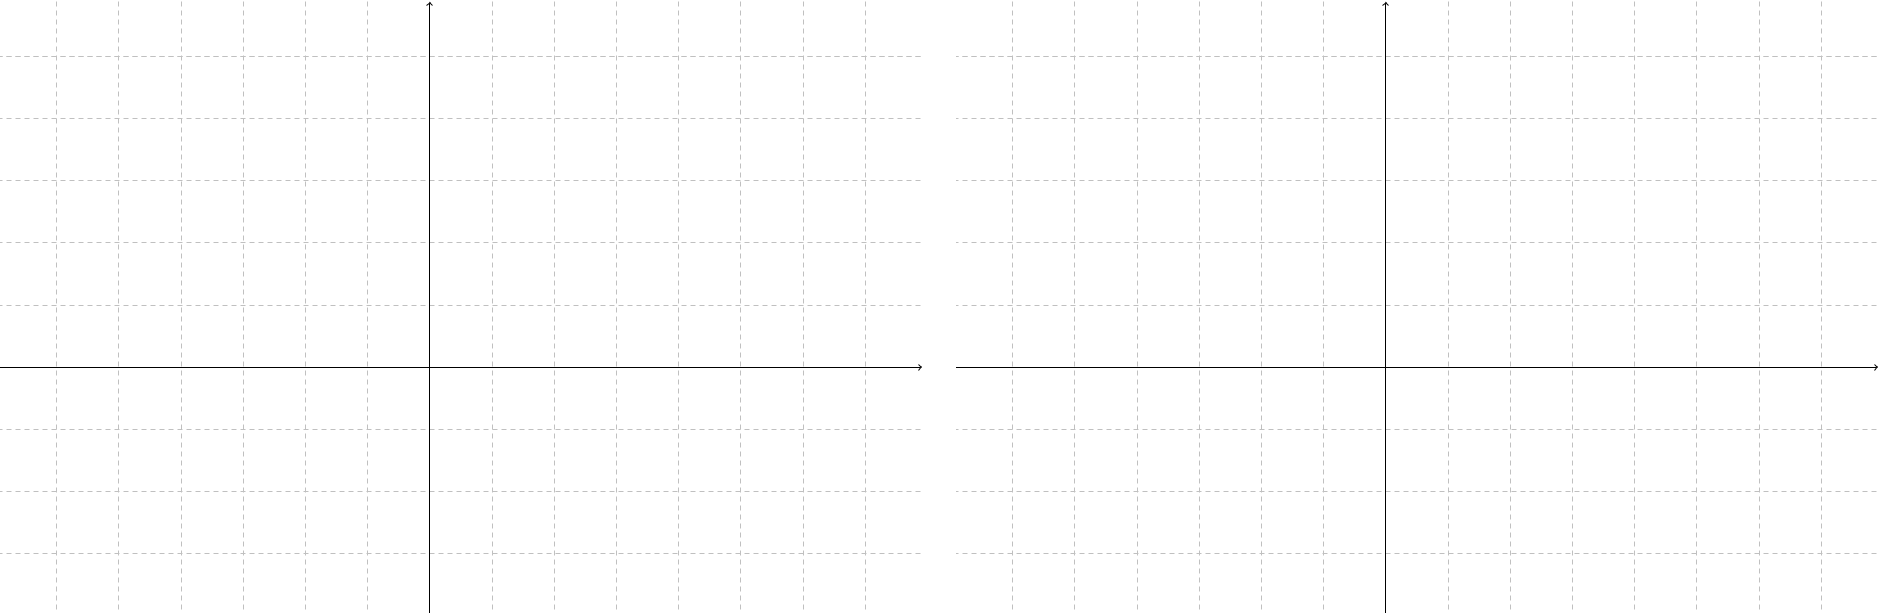
\includegraphics[width=\textwidth]{./img/c7q1.png}
\end{figure}

\begin{figure}[h]
\centering
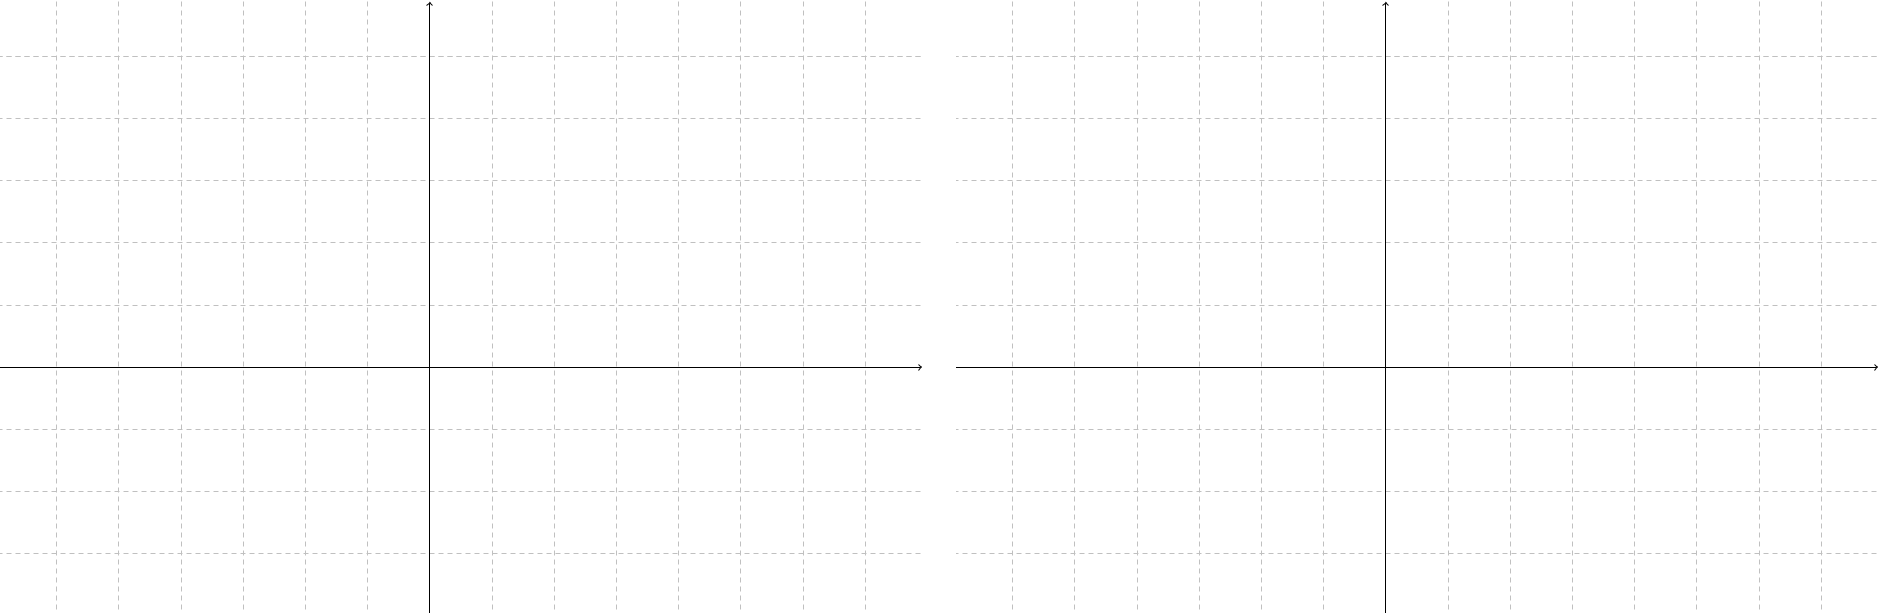
\includegraphics[width=\textwidth]{./img/c7q1.png}
\end{figure}

\begin{figure}[h]
\centering
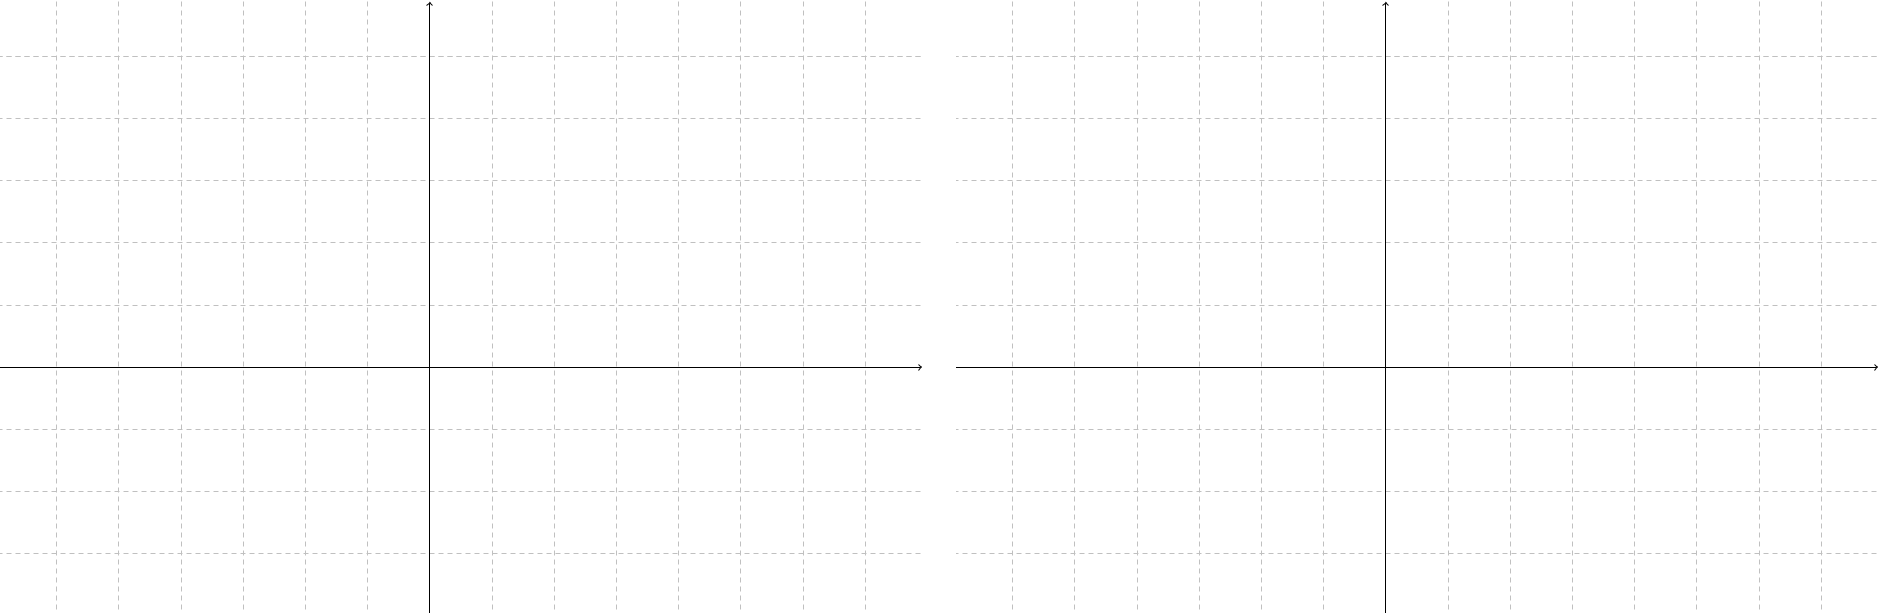
\includegraphics[width=\textwidth]{./img/c7q1.png}
\end{figure}

\newpage


\subsection*{Falando sobre gráficos}

Existem três conceitos que são muito utilizados para descrever o gráfico de funções ou trechos específicos destes: crescente, decrescente e concavidade.

Esses três conceitos podem ser definidos formalmente e, dada uma função na sua forma algébrica, é possível demonstrar qual deles se aplica ao comportamento da função em um determinado ponto. Porém, aqui faremos uma abordagem mais intuitiva e visual, uma vez que a abordagem formal será feita na disciplina de Cálculo.

Um detalhe importante: ao avaliarmos visualmente o gráfico de uma função devemos ``ler'' o gráfico da esquerda para a direita (valores de $x$ aumentando).

Dizemos que um trecho de um gráfico de uma função é \textbf{crescente} quando os valores de $y$ aumentam a medida que os de $x$ aumentam. Em termos gráficos, o segmento de curva em questão deve estar subindo (se analisarmos da esquerda pra direita). Por exemplo, o gráfico de $i(x)=\sqrt{x}$ é crescente em todo o seu domínio (volte e cheque se você concorda com essa afirmação), enquanto o gráfico de $j(x)=\sin(x)$ é crescente em alguns trechos (como o intervalo em que ele corta o eixo $Y$, de $-\pi/2$ a $\pi/2$) e não em outros.

Um exemplo de trecho \textbf{decrescente} ocorre na função $g(x)=x^2$,  quando $x<0$. Note que a curva nessa parte está descendo (se analisarmos da esquerda pra direita). Mas isso muda assim que a função cruza a origem e ela passa a ser crescente.

\begin{questao}
Considerando os gráficos traçados anteriormente, faça o que se pede em cada item.
\begin{enumerate}[a)]
\item A função $f(x)$ é crescente ou decrescente?
\item A função $h(x)$ é crescente ou decrescente?
\item Identifique um trecho em que a função $l(x)=\cos(x)$ é crescente e outro em que ela é decrescente.
\end{enumerate}
\end{questao}

O conceito de \textbf{concavidade} surge ao compararmos o formato das gráficos de $h(x)=2^x$ e $i(x)=\sqrt{x}$. Ambos são crescentes, mas se comportam de maneira diferente: $h(x)$ fica cada vez mais vertical enquanto que $i(x)$ fica cada vez mais horizontal. A diferença entre eles está na concavidade de cada um deles. Diz-se que $h(x)=2^x$ tem concavidade positiva enquanto $i(x)=\sqrt{x}$ tem concavidade negativa.

Para distinguirmos esses dois casos visualmente, podemos traçar pequenas tangentes aos gráficos em alguns pontos. Se todas as tangentes ficarem abaixo do gráfico em um intervalo (como no gráfico à esquerda abaixo) dizemos que ela tem concavidade positiva nesse intervalo. Caso contrário, a concavidade é negativa (como no gráfico à direita abaixo).

\begin{figure}[h]
\centering
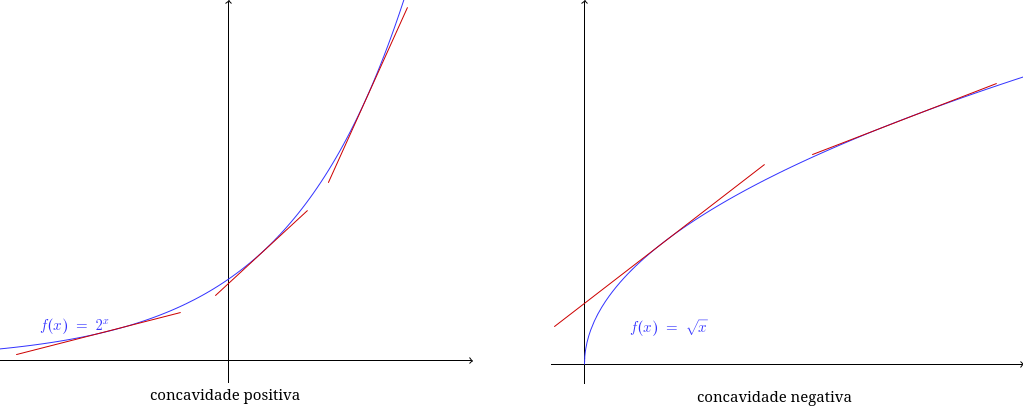
\includegraphics[width=0.9\textwidth]{./img/c7q2.png}
\end{figure}

\begin{questao}
Considerando os gráficos traçados no começo deste capítulo, faça o que se pede em cada item.
\begin{enumerate}[a)]
\item Qual é a concavidade da função $g(x)$? Ela mantém essa mesma concavidade para todo o seu domínio?
\item Identifique um trecho em que a função $j(x)=\sin(x)$ tem concavidade positiva e outro com concavidade negativa.
\end{enumerate}
\end{questao}

\subsection*{Aviso}

Deste ponto em diante, os gráficos devem ser esboçados no seu caderno. Sugerimos que use \textbf{caneta} para traçar os eixos e \textbf{lápis} para esboçar as curvas obtidas.

Além disso, todas as questões a seguir dependem da comparação de novos gráficos com os gráficos feitos na questão 1. Para facilitar a comparação, sugerimos que você use a \textbf{mesma escala} utilizada para esboçar o gráfico de referência.

Maiss uma vez, não tenha pressa ao resolver as questões a seguir. Se for necessário, faça uma tabela de valores, marque alguns pontos e então esboce o gráfico.

\subsection*{Negativo}

Vamos começar investigando o que ocorre com o gráfico de funções quando introduzimos sinais de negativo em suas expressões. Tecnicamente, o que estamos fazendo é multiplicando a função como um todo ou a variável por $-1$.

\begin{questao}
Usando como referência o gráfico de $h(x)$:
\begin{enumerate}[a)]
\item Esboce o gráfico das funções $a(x)=-(2^x)$ e $b(x)=2^{-x}$?
\item Como você descreveria o impacto causado pela multiplicação da função como um todo por $-1$ ($a(x)=-(2^x)$)?
\item Como você descreveria o impacto causado pela multiplicação da variável por $-1$ ($b(x)=2^{-x}$)?
\end{enumerate}
\end{questao}

\subsection*{Soma de constante à função}

\begin{questao}
Usando como referência o gráfico de $i(x)$:
\begin{enumerate}[a)]
\item Esboce o gráfico da função $c(x)=\sqrt{x}+2$.
\item Descreva o efeito gráfico de somarmos uma constante a uma função dada.
\item Descreva com suas palavras, sem esboça-lo, como seria o gráfico da função $c(x)=\sqrt{x}-1$ em relação ao gráfico de $i(x)$.
\end{enumerate}
\end{questao}

\subsection*{Multiplicação da função por uma constante}

\begin{questao}
Usando como referência o gráfico de $l(x)$:
\begin{enumerate}[a)]
\item Esboce o gráfico da função $d(x)=2\cos(x)$.
\item Descreva o efeito gráfico de multiplicarmos uma função dada por uma constante.
\item O que ocorrerá se a constante for positiva, mas menor do que 1?
\end{enumerate}
\end{questao}

\subsection*{Mais casos envolvendo somas}

\begin{questao}
Usando como referência o gráfico de $g(x)$:
\begin{enumerate}[a)]
\item Esboce os gráficos das funções $p(x)=x^2+1$ e $q(x)=(x+1)^2$.
\item Descreva o que aconteceu com o gráfico de $p(x)$.
\item Descreva o que aconteceu com o gráfico de $q(x)$.
\item Qual é a diferença do que foi feito com $g(x)$ para obter $p(x)$ e $q(x)$?
\item Qual transformação deve ser feita na função $e(x)=\sin(x)$ para que o seu gráfico se desloque horizontalmente 2 unidades para a direita?
\end{enumerate}
\end{questao}

\subsection*{Outra multiplicação}

\begin{questao}
Usando como referência o gráfico de $e(x)$:
\begin{enumerate}[a)]
\item Esboce os gráficos das funções $t(x)=\sin(2x)$ e $u(x)=\sin(2\pi x)$.
\item Qual é o período de cada uma das funções?
\item Como você descreveria o efeito na função seno de multiplicarmos a variável por uma constante?
\end{enumerate}
\end{questao}

\subsection*{Finalização}

Nas questões anteriores você pôde visualizar o efeito que quatro transformações algébricas diferentes:

\begin{itemize}
 \item multiplicar a função por uma constante;
 \item multiplicar a variável por uma constante;
 \item somar uma constante à função;
 \item somar uma constante à variável.
\end{itemize}

Cada uma dessas transformações algébricas causa um efeito geométrico no gráfico da função. Esses efeitos são mais simples de visualizar em algumas funções específicas, sendo bem difíceis de visualizar em outros casos. 

Poderíamos fazer uma lista dos transformações e seus efeitos para que você decorasse e soubesse identificar rapidamente certas características de certas funções, porém, não é esse o foco deste material. O que pretendemos é que você saiba que transformações algébricas como soma e multiplicação, seja da função como um todo ou da variável, têm efeitos previsíveis no gráfico da função e que esses efeitos são essencialmente de dois tipos:

\begin{itemize}
 \item deslocamento (vertical ou horizontal);
 \item encolhimento/esticamento (vertical ou horizontal).
\end{itemize}

Ter esses efeitos em mente deve facilitar o seu trabalho quando você também utilizar derivadas para esboçar o gráfico de uma função dada.

Na questão a seguir, você deverá esboçar quatro gráficos em um mesmo eixo cartesiano. Muito mais importante do que a precisão e os detalhes dos gráficos, é a possibilidade de compararmos o comportamento geral de um com o outro.

\begin{questao}
Esboce em um mesmo eixo cartesiano e \textbf{sem utilizar uma tabela de valores} o gráfico das quatro funções abaixo. Sugestão: use 4 cores diferentes.
\begin{enumerate}[a)]
\item $j_a (x)=2\sin(x)$
\item $j_b (x)=\sin(\frac{x}{4})$
\item $j_c (x)=\sin(x)-1$
\item $j_d (x)=\sin(x+\pi)$
\end{enumerate}
\end{questao}

\newpage

\section{Rumo ao livro-texto}

A questão abaixo foi retirada da seção 1.3 do livro \sugestao{Calculus}, de James Stewart. Pode parecer um retrocesso em termos de conteúdo voltar para o primeiro capítulo do livro, mas essa seção está fortemente ligada ao que será discutido no capítulo 4 e ao que discutimos neste capítulo.

\begin{resolvida}
O gráfico de $y=f(x)$ é dado abaixo associe as expressões algébricas abaixo ao outros gráficos dados e dê uma razão para as suas escolhas.

\begin{figure}[h]
\centering
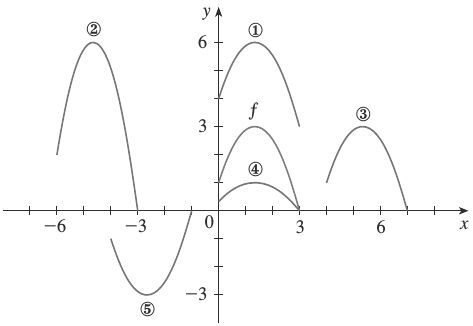
\includegraphics[width=0.6\textwidth]{./img/c7r1.png}
\end{figure}

\begin{enumerate}[a)]
\item $y=f(x-4)$
\item $y=f(x)+3$
\item $y= \frac{1}{3}f(x)$
\item $y=-f(x+4)$
\item $y=2f(x+6)$
\end{enumerate}
\end{resolvida}

%PREFACE: Eu usei textit pra diferenciar quando estou falando dos elementos da imagem e quando estou falando de números. Vejam como resolver isso, a intencao era apenas fazer esse distincao.
Nessa questão, a expressão algébrica da função não foi dada, apenas o seu gráfico. Note que o gráfico $f$ está definido apenas no intervalo de $0$ a $3$. Algumas outras conclusões podem ser tiradas facilmente do gráfico, como $f(0)=1$, $f(3)=0$ e o valor máximo da função é $3$.

Para começarmos a identificar qual dos demais gráficos se referem a cada uma das transformações dadas, vamos começar com os gráficos mais parecidos com o de $f$. Na minha opinião, \textit{1} e \textit{3} são os mais simples, pois ambos parecem ter exatamente o mesmo formato e estarem apenas deslocados horizontalmente ou verticalmente. Começando por \textit{1}, os valores da função parecem ser exatamente $3$ unidades maiores do que $f$, ou seja, teríamos que somar $3$ à função, ou seja, o gráfico \textit{1} corresponde à expressão \textit{b}.

Por outro lado, o gráfico \textit{3} foi deslocado $4$ unidades para a direita, o que é compatível com a expressão \textit{a}.

O gráfico \textit{4} parece não ter sido deslocado, apenas ``achatado''. Note que o máximo da função passou a ser $1$ ao invés de $3$. Esse efeito é alcançado ao dividirmos a função por $3$, o que é compatível com a expressão \textit{c}.

Nos restam os gráficos \textit{5} e \textit{2}. Note que o gráfico \textit{5} está refletido, além de ter sido deslocado. Sabemos que um gráfico é refletido verticalmente quando a função como um todo é multiplicada por $-1$, e isso é compativel com a expressão \textit{d}.

Portanto, o gráfico \textit{2} deve vir da expressão \textit{e}. Isso é coerente, pois esse gráfico foi claramente ``esticado'' verticalmente, o que é compatível com a expressão \textit{e}.

Agora, resolva a questão a seguir, retirada da mesma seção do livro \sugestao{Calculus}.

\begin{resolva}
O gráfico de $f$ é dado abaixo. Esboce o gráfico das seguintes funções:

\begin{figure}[h]
\centering
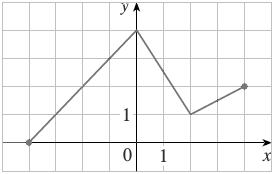
\includegraphics[width=0.6\textwidth]{./img/c7r2.png}
\end{figure}

\begin{enumerate}[a)]
\item $y=f(x+4)$
\item $y=f(x)+4$
\item $y=2f(x)$
\item $y= -\frac{1}{2}f(x)+3$
\end{enumerate}
\end{resolva}

\newpage

\section{Gabarito}

Confira as respostas para as questões e \textbf{não se esqueça de registrar o seu progresso}.

Questões sobre esboço de gráficos não terão gabarito, com exceção da questão 10.

\noindent\textbf{Questão 1:} Questão sem gabarito. Cheque a lista logo após a questão para cobrir características básicas de cada gráfico e pergunte a seu tutor se os esboços estão bons.

\noindent\textbf{Questão 2:} a) crescente, b) $g(x)$ é decrescente para $x<0$ e crescente para $x>0$.

\noindent\textbf{Questão 3:} a) concavidade positiva, b) no intervalo $0x<\pi$.

\noindent\textbf{Questão 4:} b) O gráfico foi refletido verticalmente, ou seja, em relação ao eixo $X$, c) O gráfico foi refletido horizontalmente, ou seja, em relação ao eixo $Y$.

\noindent\textbf{Questão 5:} b) o gráfico da função se desloca verticalmente, c) o gráfico se deslocaria para baixo, passando a assumirmos alguns valores positivos. Seu mínimo seria em $(0;-1)$ e raiz em $(1;0)$.

\noindent\textbf{Questão 6:} b) O gráfico da função é esticado verticalmente, b) O gráfico será encolhido verticalmente, c) O gráfico será refletido verticalmente e depois encolhido ou esticado, dependendo do módulo da constante.

\noindent\textbf{Questão 7:} b) Foi deslocado uma unidade para cima, c) Foi deslocado uma unidade para a esquerda, c) em $p(x)$ a constante foi soma à função e em $q(x)$ à variável, d) $e(x)=\sin(x-2)$.

\noindent\textbf{Questão 8:} b) O periodo de $t(x)$ é $\pi$ e o de $u(x)$ é $1$, c) O gráfico da função é encolhido horizontalmente. Se a função for periódica, podemos dizer que o seu período foi alterado.

\noindent\textbf{Questão 9:} a) $j_a(x)=2\sin(x)$, b) $j_b(x)=\sin(x/4)$, c)$j_c(x)=\sin(x)-1$, $j_d(x)=\sin(x+\pi)$.

\noindent\textbf{Questão 10:}

\begin{figure}[h]
\centering
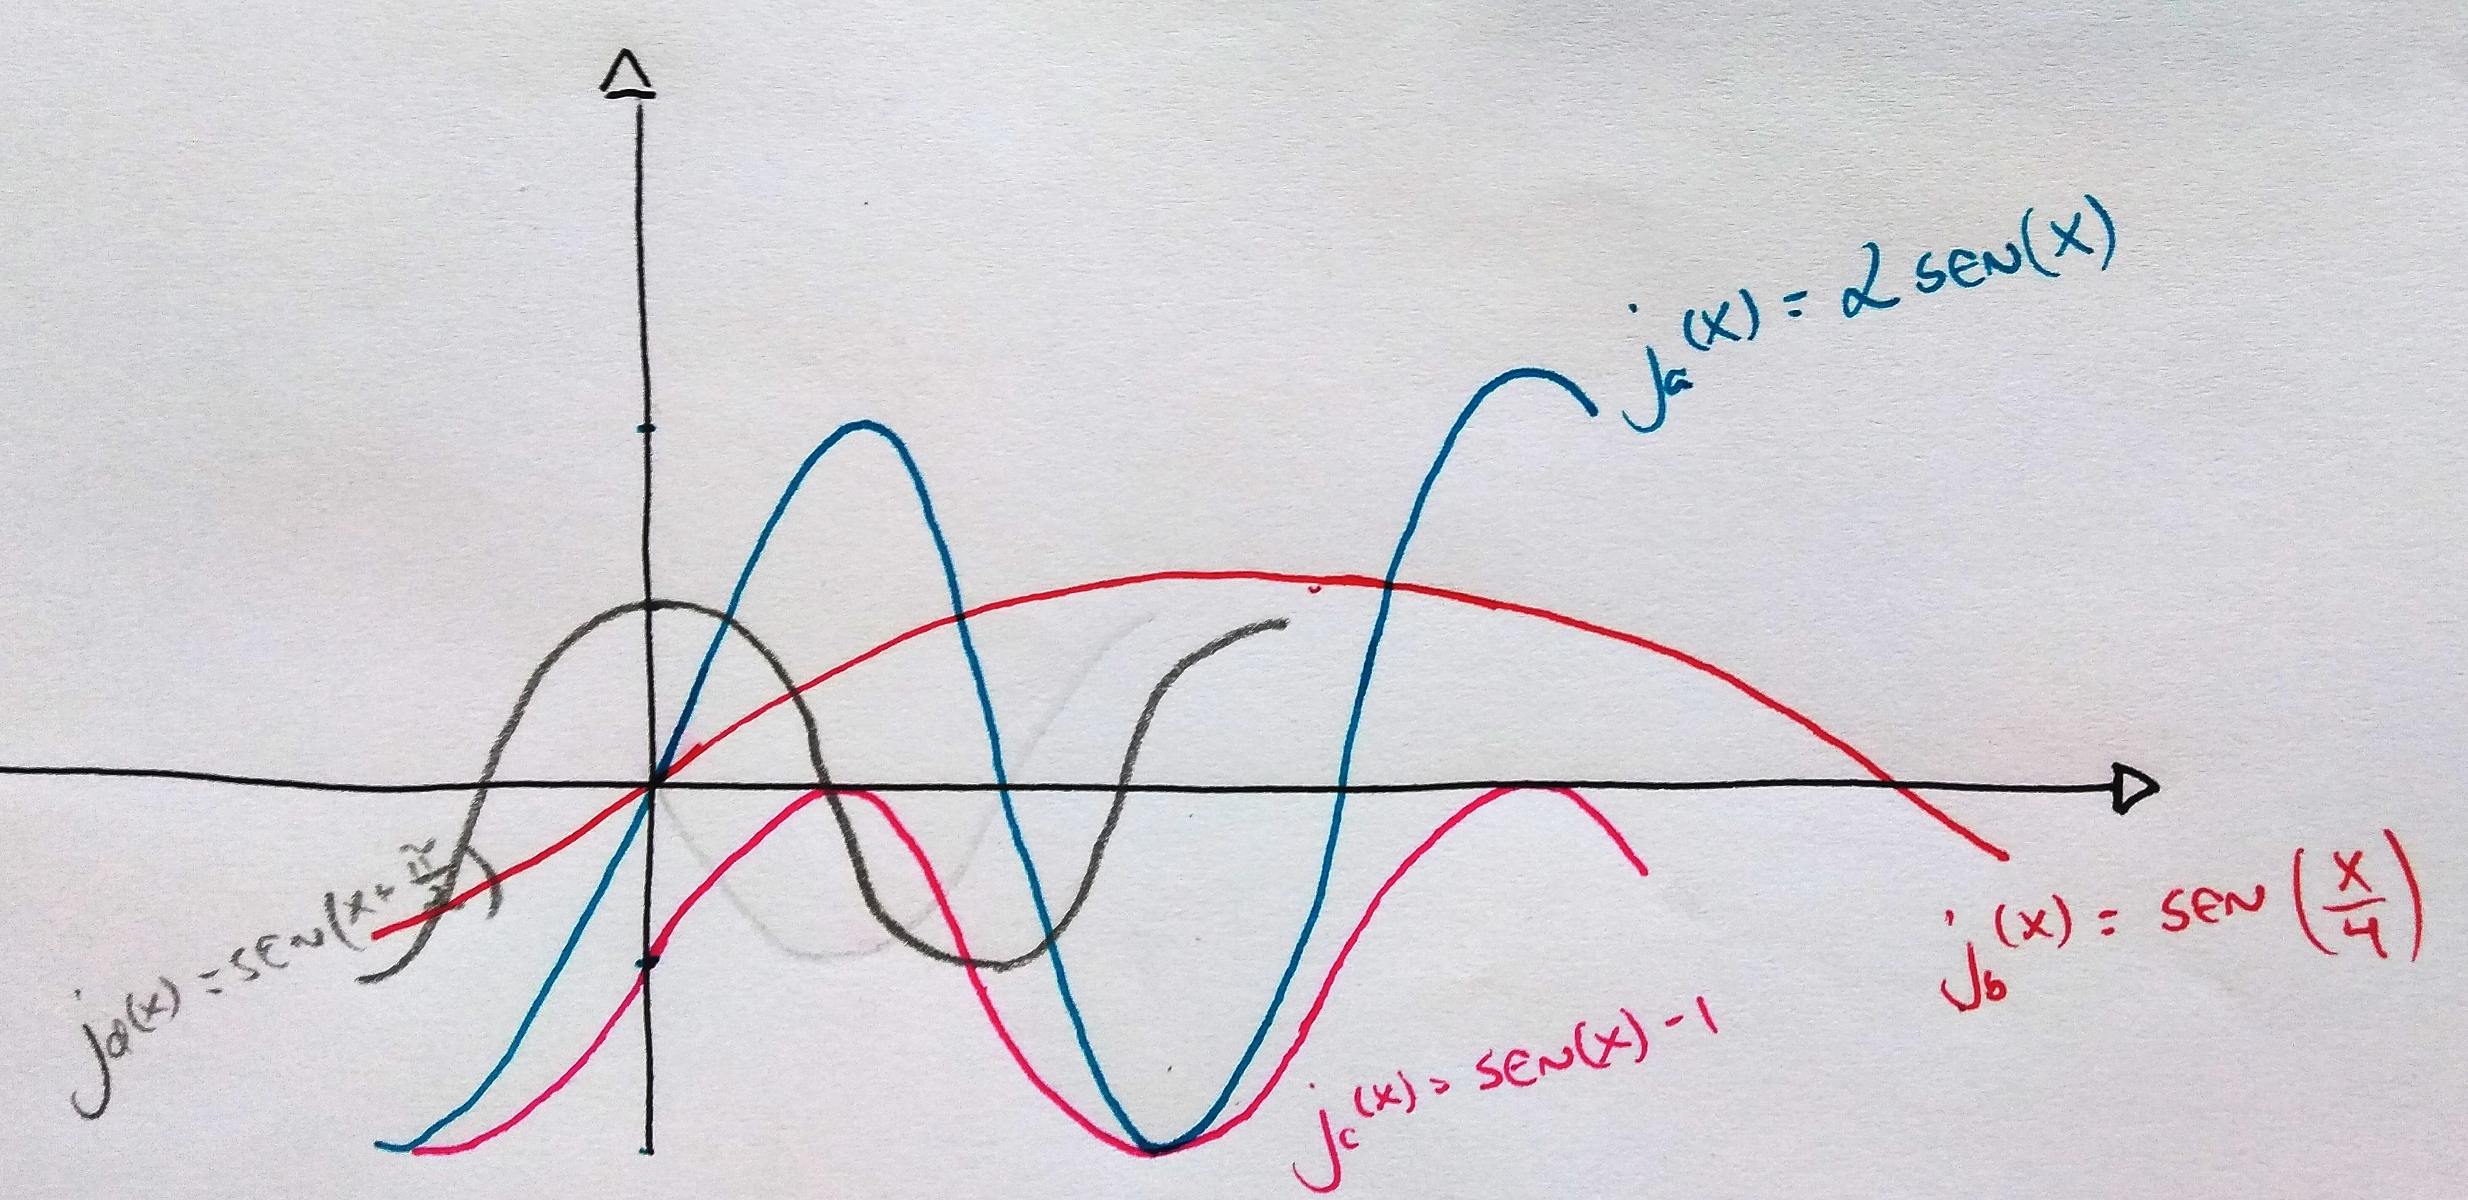
\includegraphics[width=0.75\textwidth]{./img/c7g10.jpg}
\end{figure}

\newpage

\section{Registro de progresso}

Essa parte por enquanto fica com conteúdo vazio até que seja decidido como será feito o controle do progresso.
\vspace{5cm}

\section{Auto-avaliação final}
Avalie o quanto você acha que sabe sobre os seguintes itens após ter resolvido as questões deste capítulo.

\begin{center}
 \begin{tabular}{|p{35mm}||p{15mm}|p{15mm}|p{15mm}|p{15mm}|} 
 \hline
   & Nada & Muito pouco & Noções gerais & Bastante\\
 \hline
 Traçar o gráfico de uma função simples &  &  &  &  \\ 
 \hline
 Deslocar o gráfico de uma função no plano cartesiano &  &  &  &  \\
 \hline
 Obter a expressão algébrica de uma função a partir do seu gráfico &  &  &  &  \\
 \hline
\end{tabular}
\end{center}

Cheque como foi o seu progresso comparando essas respostas com as que você deu antes de estudar este capítulo. Caso você não tenha atingido o nível ``Bastante''  em algum dos tópicos acima, liste abaixo qual ação concreta você fará nos próximos dias para atingi-lo:

\vspace{0.3cm}

\noindent\rule{\linewidth}{0.4pt}

\noindent\rule{\linewidth}{0.4pt}

\noindent\rule{\linewidth}{0.4pt}

\end{document}
